% This is a Basic Assignment Paper but with like Code and stuff allowed in it, there is also url, hyperlinks from contents included. 

\documentclass[11pt]{article}

% Preamble

\usepackage[margin=1in]{geometry}
\usepackage{amsfonts, amsmath, amssymb}
\usepackage{fancyhdr, float, graphicx}
\usepackage[utf8]{inputenc} % Required for inputting international characters
\usepackage[T1]{fontenc} % Output font encoding for international characters
\usepackage{fouriernc} % Use the New Century Schoolbook font
\usepackage[nottoc, notlot, notlof]{tocbibind}
\usepackage{listings}
\usepackage{xcolor}
\usepackage{blindtext}
\usepackage{hyperref}
\hypersetup{
    colorlinks=true,
    linkcolor=black,
    filecolor=magenta,      
    urlcolor=cyan,
    pdfpagemode=FullScreen,
    }

\definecolor{codegreen}{rgb}{0,0.6,0}
\definecolor{codegray}{rgb}{0.5,0.5,0.5}
\definecolor{codepurple}{rgb}{0.58,0,0.82}
\definecolor{backcolour}{rgb}{0.95,0.95,0.92}

\lstdefinestyle{mystyle}{
    backgroundcolor=\color{backcolour},   
    commentstyle=\color{codegreen},
    keywordstyle=\color{magenta},
    numberstyle=\tiny\color{codegray},
    stringstyle=\color{codepurple},
    basicstyle=\ttfamily\footnotesize,
    breakatwhitespace=false,         
    breaklines=true,                 
    captionpos=b,                    
    keepspaces=true,                 
    numbers=left,                    
    numbersep=5pt,                  
    showspaces=false,                
    showstringspaces=false,
    showtabs=false,                  
    tabsize=2
}

\lstset{style=mystyle}

% Header and Footer
\pagestyle{fancy}
\fancyhead{}
\fancyfoot{}
\fancyhead[L]{\textit{\Large{OOPJC Mini Project Report}}}
%\fancyhead[R]{\textit{something}}
\fancyfoot[C]{\thepage}
\renewcommand{\footrulewidth}{1pt}



% Other Doc Editing
% \parindent 0ex
%\renewcommand{\baselinestretch}{1.5}

\begin{document}

\begin{titlepage}
	\centering

	%---------------------------NAMES-------------------------------

	\huge\textsc{
		MIT World Peace University
	}\\

	\vspace{0.75\baselineskip} % space after Uni Name

	\LARGE{
		NASA Space Apps Challenge 2023
	}

	\vfill % space after Sub Name

	%--------------------------TITLE-------------------------------

	\rule{\textwidth}{1.6pt}\vspace*{-\baselineskip}\vspace*{2pt}
	\rule{\textwidth}{0.6pt}
	\vspace{0.75\baselineskip} % Whitespace above the title



	\huge{\textsc{
			STAR App LLM for Querying Technical Documentation.
		}} \\


	\vspace{0.5\baselineskip} % Whitespace below the title
	\rule{\textwidth}{0.6pt}\vspace*{-\baselineskip}\vspace*{2.8pt}
	\rule{\textwidth}{1.6pt}

	\vspace{1\baselineskip} % Whitespace after the title block

	%--------------------------SUBTITLE --------------------------	

	\LARGE\textsc{
		NASA Space Apps Challenge 2023
	} % Subtitle or further description
	\vfill

	%--------------------------AUTHOR-------------------------------

	Prepared By
	\vspace{0.5\baselineskip} % Whitespace before the editors

	\Large{
		Krishnaraj Thadesar \\
		Sahaj Mishra \\
		Neeraj Verma  \\
		Saubhagya Singh \\
		Aaron Philip \\
		Yashwardhan Tekawade \\
	}


	\vspace{0.5\baselineskip} % Whitespace below the editor list
	\today

\end{titlepage}


\tableofcontents
\thispagestyle{empty}
\clearpage

\setcounter{page}{1}

\section{Problem Statement}

\textit{Greetings, space enthusiast! Are you tired of slogging through technical requirements, only to find omissions and inconsistencies that could spell disaster for your mission? What if there was an Artificial Intelligence (AI)-powered app called STAR (Standards Technical Assistance Resource) that could streamline the process and offer requirement recommendations? Your challenge is to develop the approach, code, or procedure for STAR, so that with STAR as a copilot, mission designers can blast off with even greater confidence, knowing that they have the right requirements in place.}

\section{Screenshots}

\subsection{Login}
\begin{figure}[H]
	\centering
	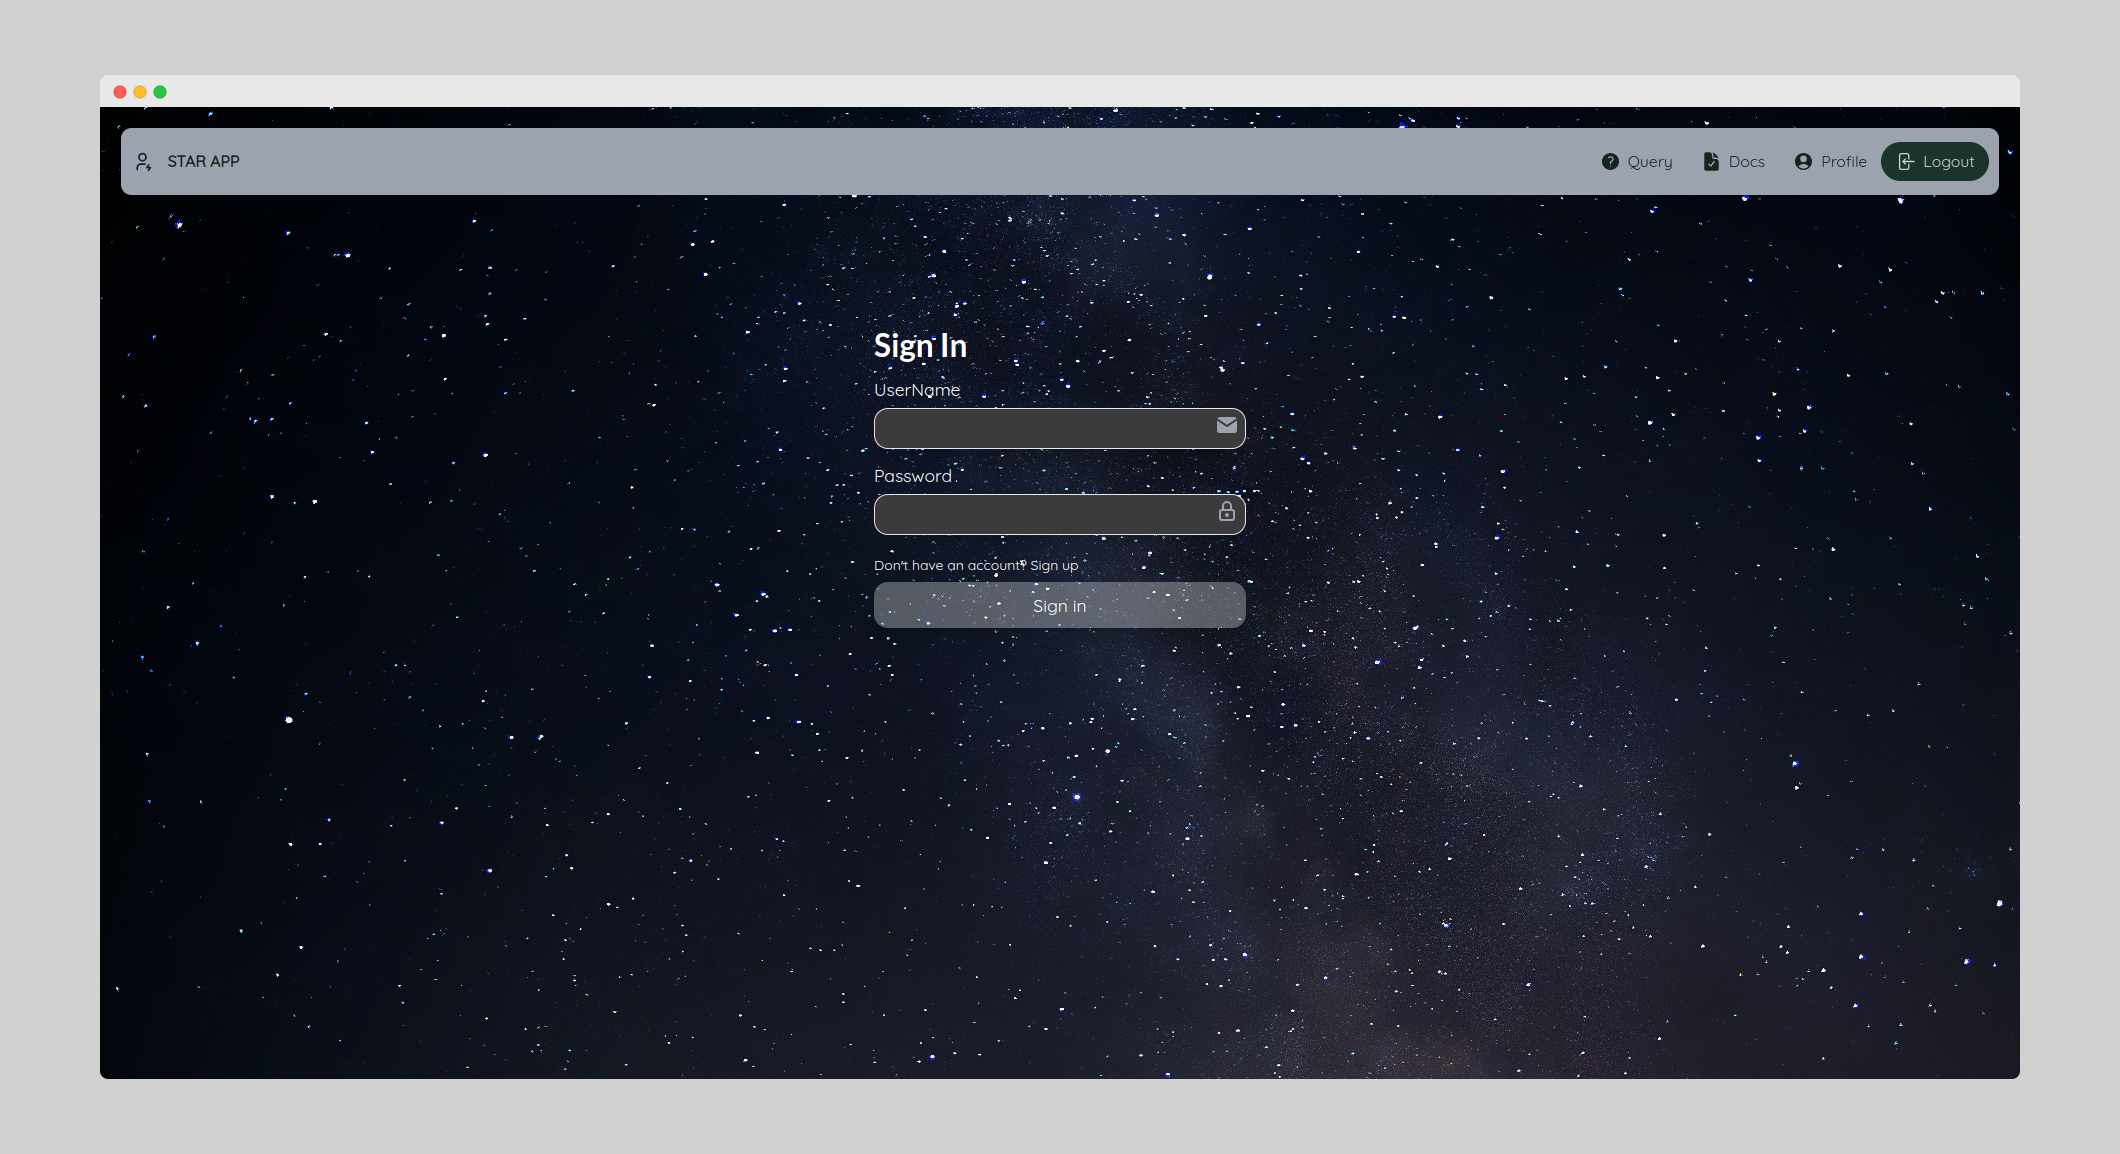
\includegraphics[width=.95\textwidth]{./signin.png}
	\caption{signin}
\end{figure}
\subsection{Query Page}
\begin{figure}[H]
	\centering
	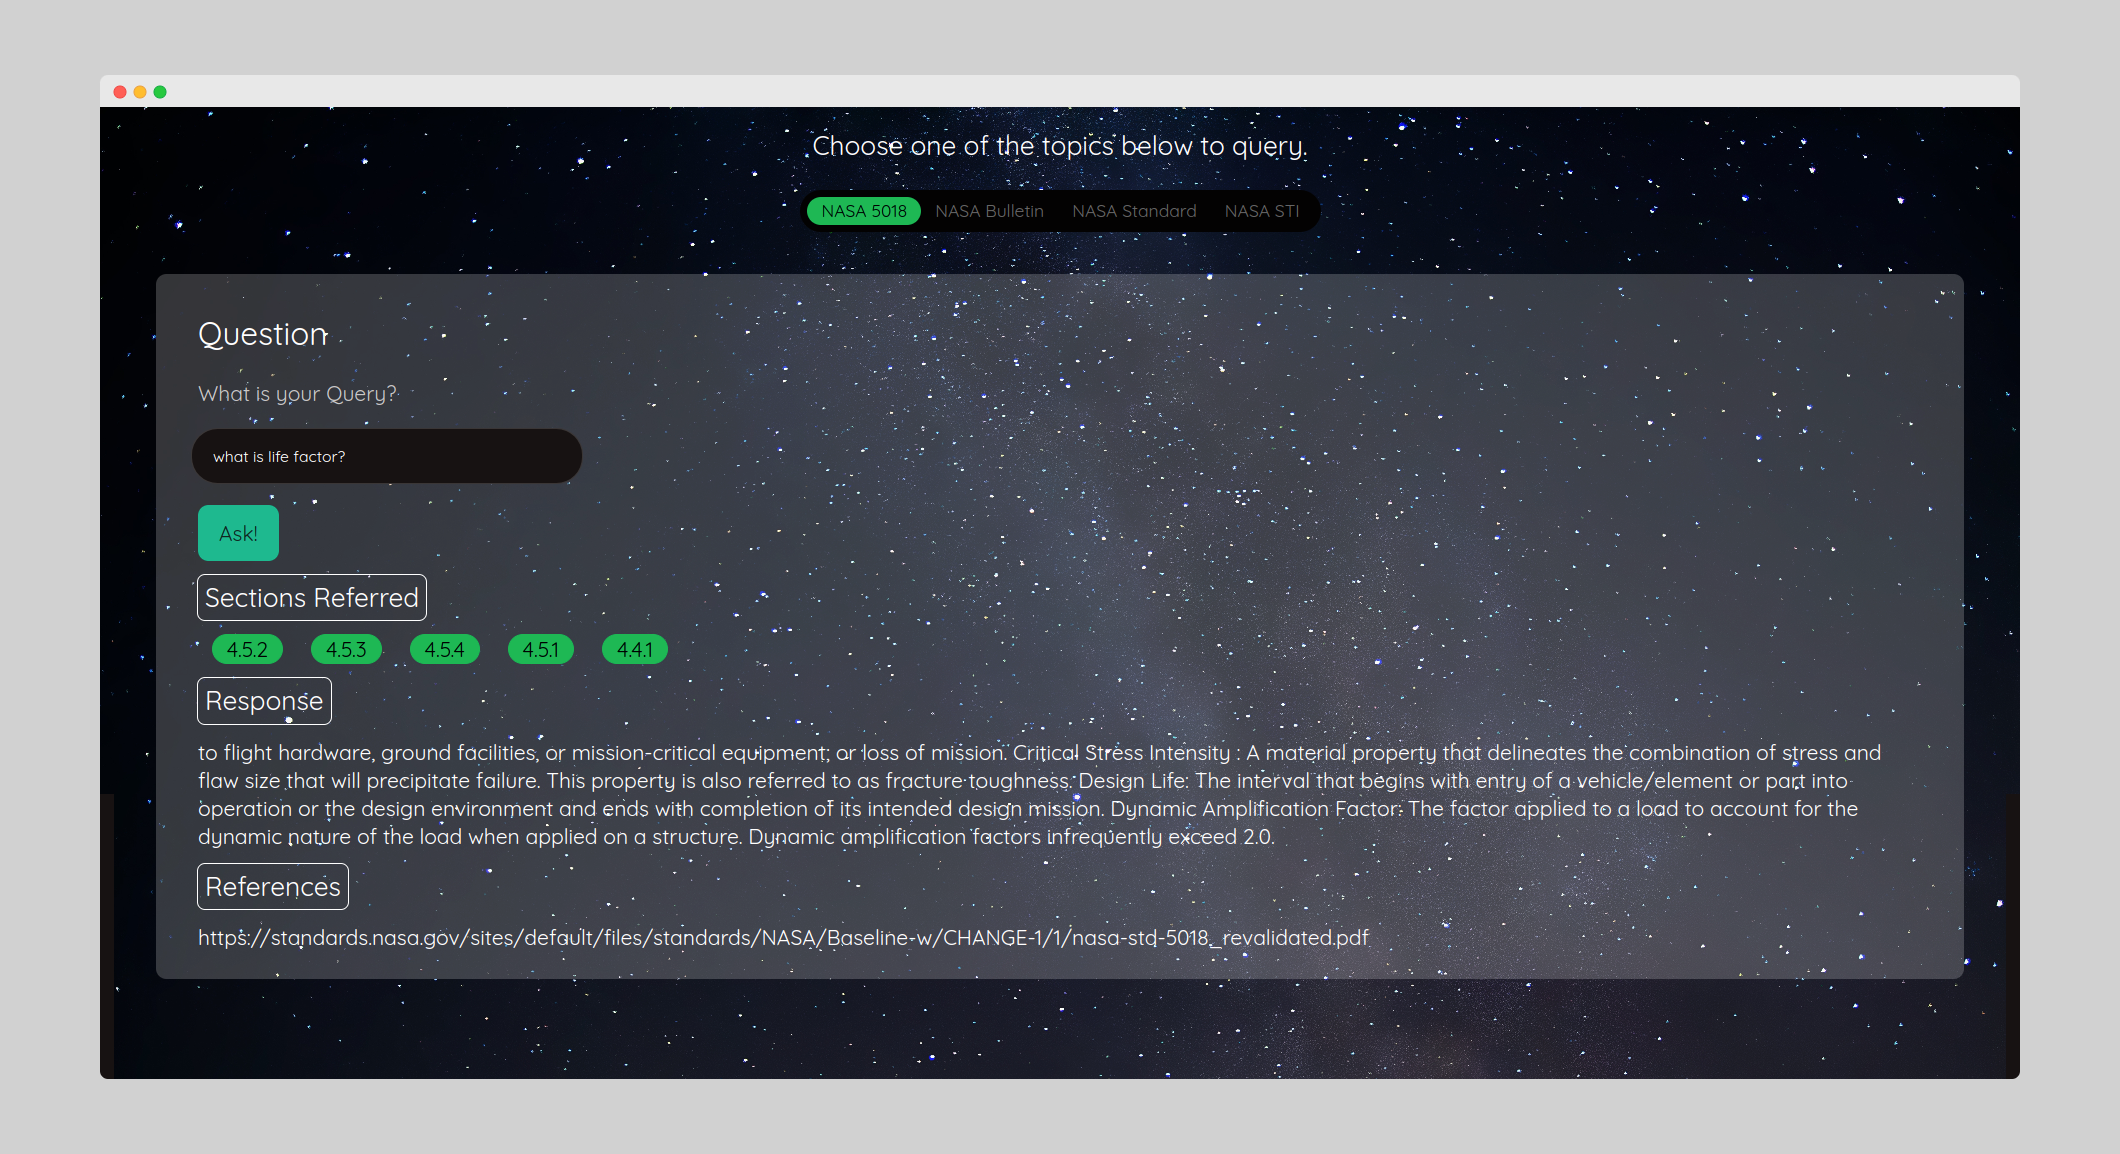
\includegraphics[width=.95\textwidth]{./answer.png}
	\caption{Query}
\end{figure}
\subsection{Answer}
\begin{figure}[H]
	\centering
	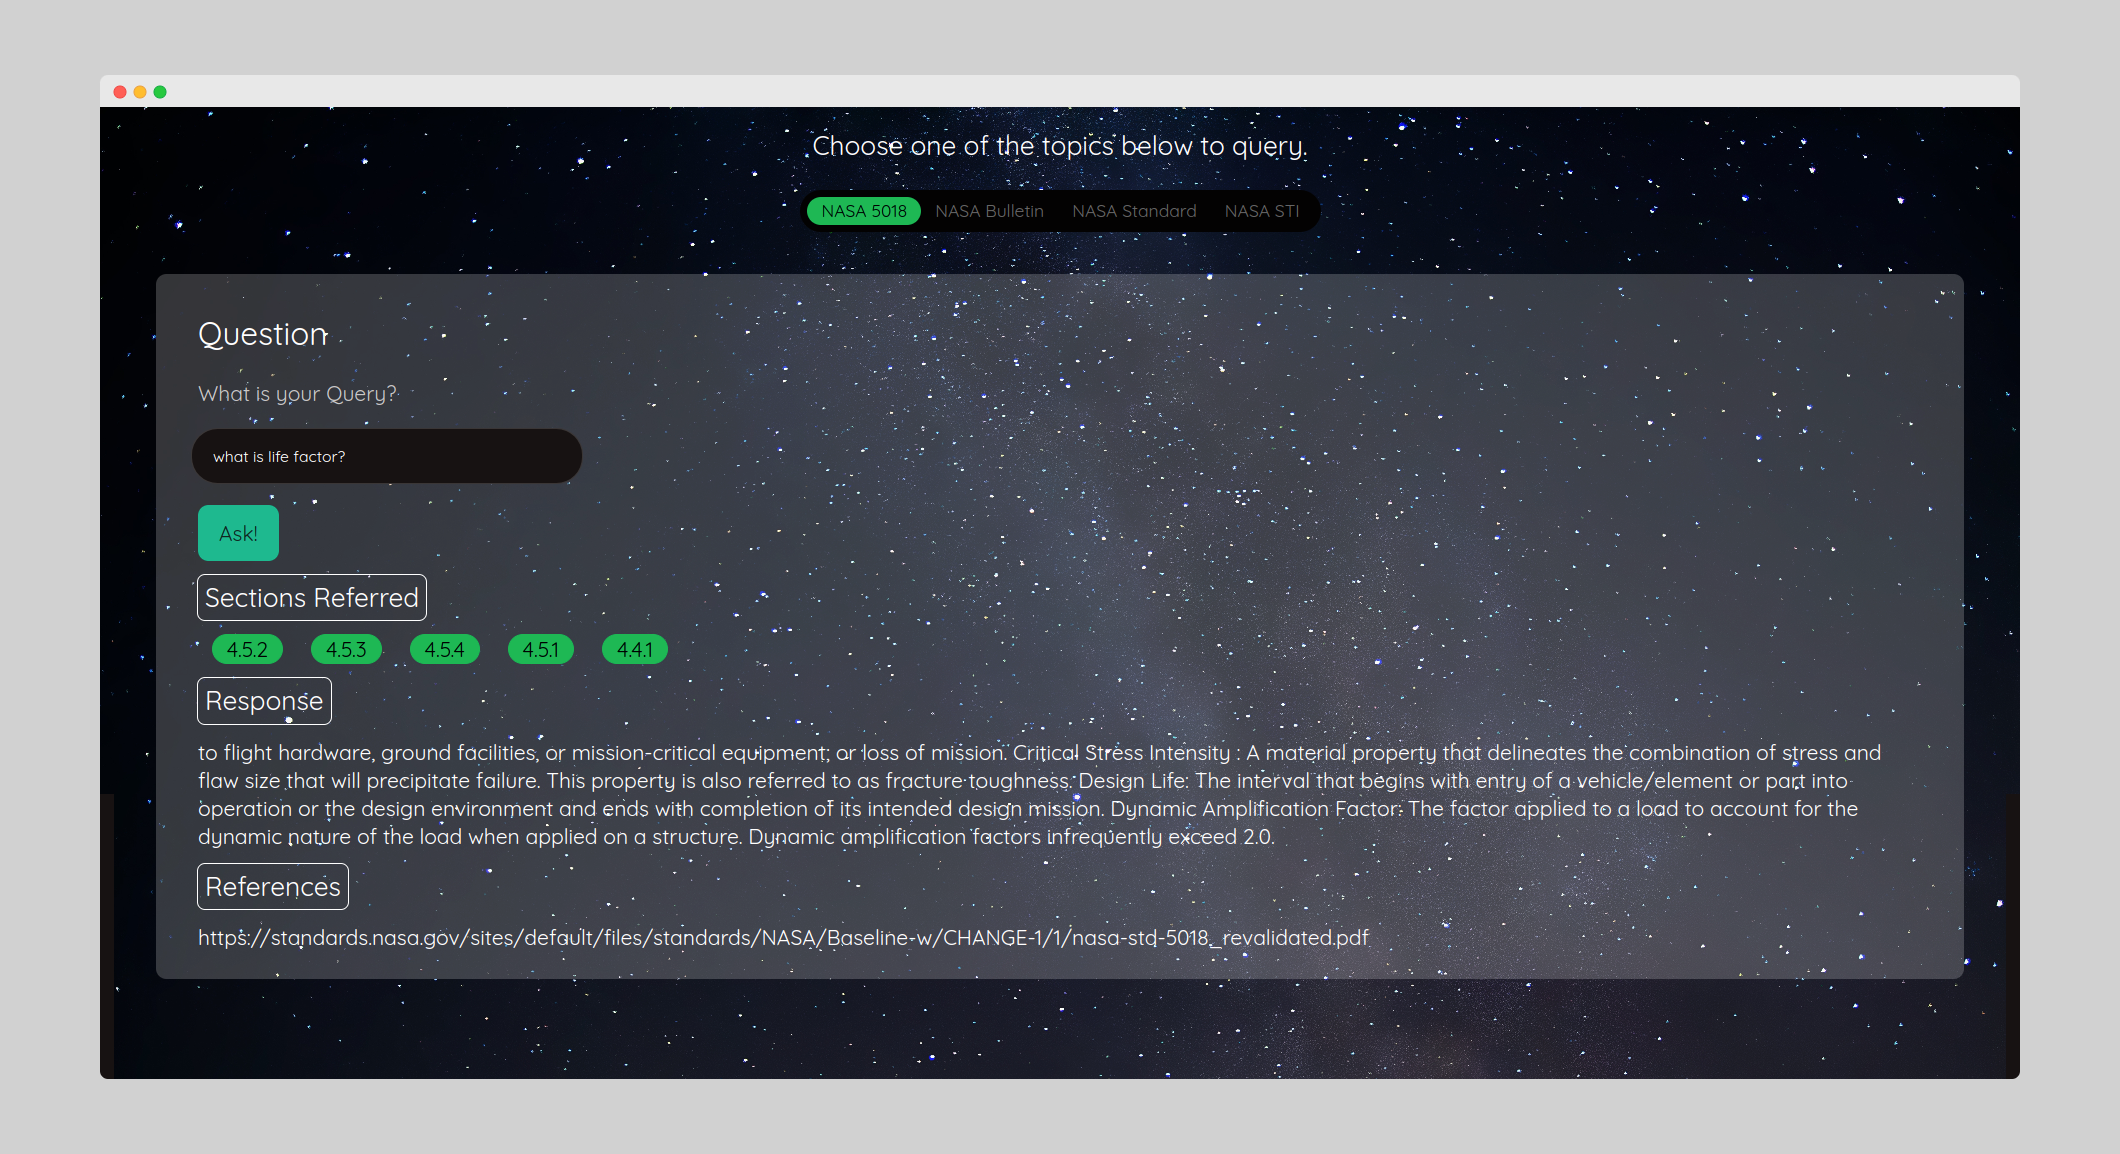
\includegraphics[width=.95\textwidth]{./answer.png}
	\caption{Answer}
\end{figure}
\subsection{Docs}
\begin{figure}[H]
	\centering
	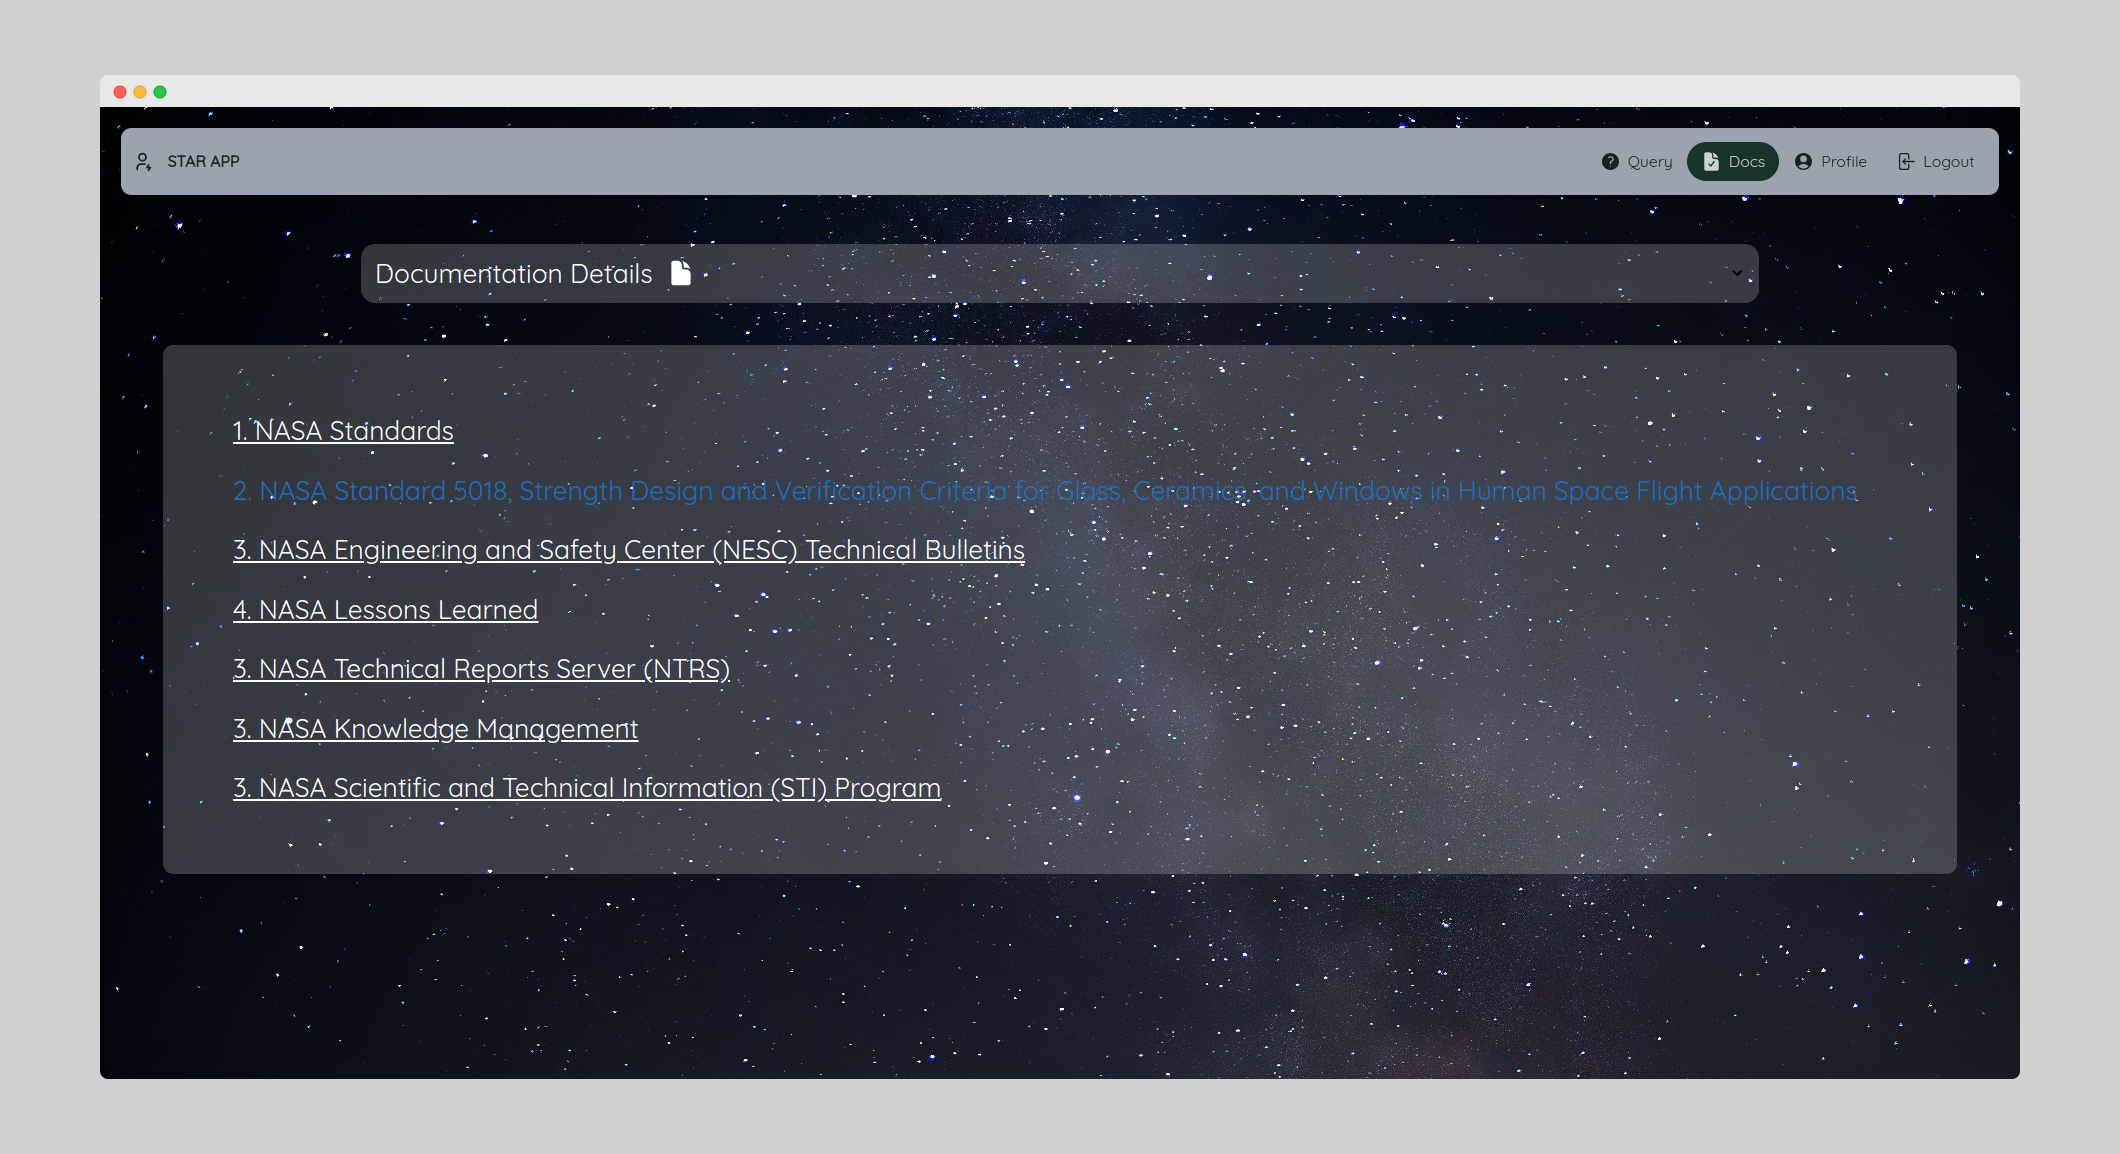
\includegraphics[width=.95\textwidth]{./doc.png}
	\caption{Docs}
\end{figure}

\section{Features}
\begin{enumerate}
	\item Ability to ingest and convert documents into queryable information
	\item Ability to text with the contents of the document
	\item Different document sources to choose from
	\item Ability to view previous queries of a user
	\item User authentication and security
	\item Ability to view source documents directly
	\item Segmented answers that provide section,response,ref
	\item Interactive UI
	\item Dark mode
\end{enumerate}

\section{Files and Directories}

\subsection{Backend}
\subsubsection{views.py}

\begin{enumerate}
	\item The file defines several functions for user registration, login, and querying NASA-related information.
	\item The functions use various libraries such as Django, faiss, and bcrypt for authentication and data retrieval.
	\item The functions retrieve relevant documents based on user queries and return the answers, sections, and references as a JSON response.
	\item The file also includes a function to remove special characters from text and a function to retrieve user query data from the database.
	\item The file uses regular expressions to match patterns in the retrieved documents and extract relevant information.
\end{enumerate}

\subsubsection{registeruser}
\begin{enumerate}
	\item The code defines a function called registeruser that handles user registration requests.
	\item The function checks if the request method is POST and parses the request body as JSON data.
	\item The function validates the email format and checks if the required fields (username, password, and email) are present in the request data.
	\item The function concatenates the username and password, hashes the concatenated value using bcrypt, and inserts the user data into a database table called UserReltion.
	\item The function returns a JSON response indicating whether the user registration was successful or not.
\end{enumerate}
\subsubsection{loginuser}
\begin{enumerate}
	\item The code defines a function called loginuser that handles user login requests.
	\item The function checks if the request method is POST and parses the request body as JSON data.
	\item The function retrieves user data from the database based on the provided username and checks if the provided password matches the hashed password in the database.
	      If the authentication is successful, the function returns a JSON response indicating that the login was successful.
	      If the authentication fails, the function returns a JSON response indicating that the username or password is invalid, or that the user was not found in the database.
\end{enumerate}
\subsubsection{nasa}
\begin{enumerate}
	\item The code defines a function called nasa that handles NASA-related queries.
	\item The function uses the GooglePalmEmbeddings class to create embeddings for the query and the FAISS class to retrieve relevant documents based on the query.
	\item The function retrieves the query and username from the request parameters and checks if the query contains the word "summary".
	\item The function extracts relevant information from the retrieved documents using regular expressions and returns the answers, sections, and references as a JSON response.
	\item The function also has a commented-out section that appends the query to the queriesdata field in the UserReltion table in the database.
\end{enumerate}
\subsubsection{bulletin}
\begin{enumerate}
	\item The code defines a function called bulletin that handles requests related to NASA bulletins.
	\item The function uses the GooglePalmEmbeddings class to create embeddings for the query and the FAISS class to retrieve relevant documents based on the query.
	\item The function retrieves the query from the request parameters and checks if it is empty. If it is empty, the function returns a JSON response with an error message and a 400 status code.
	\item The function retrieves relevant documents based on the query and extracts relevant information using regular expressions. It then returns the answers, sections, and references as a JSON response.
	\item The function also has a commented-out section that appends the query to the queriesdata field in the UserReltion table in the database.
\end{enumerate}
\subsubsection{standards}
\begin{enumerate}
	\item The code defines a function called standards that handles requests related to NASA standards.
	\item The function creates a GooglePalmEmbeddings object and a FAISS object to retrieve relevant documents based on the query.
	\item The function retrieves the query from the request parameters and checks if it is empty. If it is empty, the function returns a JSON response with an error message and a 400 status code.
	\item The function retrieves relevant documents based on the query and extracts relevant information using regular expressions. It then returns the answers, sections, and references as a JSON response.
	\item The function returns a JSON response with the answers, sections, and references to the relevant NASA standards.
\end{enumerate}
\subsubsection{spacetech}
\begin{enumerate}
	\item The code defines a function called spacetech that handles requests related to space technology.
	\item The function creates a GooglePalmEmbeddings object and a FAISS object to retrieve relevant documents based on the query.
	\item The function retrieves the query from the request parameters and checks if it is empty. If it is empty, the function returns a JSON response with an error message and a 400 status code.
	\item The function retrieves relevant documents based on the query and extracts relevant information using regular expressions. It then returns the answers, sections, and references as a JSON response.
	\item The function returns a JSON response with the answers, sections, and references to the relevant space technology documents.
\end{enumerate}

\subsubsection{queriesrequest}

\begin{enumerate}
	\item The code defines a function called queriesreuest that handles GET requests related to user queries.
	\item The function retrieves the username from the request parameters and checks if it is empty. If it is empty, the function returns a JSON response with an error message and a 400 status code.
	\item The function retrieves query data from the database based on the provided username using a SQL query.
	\item The function extracts the query data from the SQL query result and returns it as a JSON response.
	      If the provided username is not found in the database, the function returns a JSON response with an error message and a 404 status code.
\end{enumerate}

\subsection{Frontend}


\subsection{Machine Learning}

\textbf{User Interaction} This feature involves handling interactions with the user. Users input their queries or questions through a user interface, and the bot is responsible for processing these inputs and providing relevant answers.

\textbf{Query Processing} In this step, the bot takes the user's query and prepares it for further analysis. It may involve text preprocessing, removing irrelevant information, or extracting key terms to improve the accuracy of the search.

\textbf{Query Embedding} Query embedding is a technique used to convert the user's query into a numerical vector representation. This numerical representation helps in comparing the query with other text data for similarity analysis.

\textbf{Similarity Search} Similarity search is a core component of the bot's functionality. It involves comparing the query embedding to embeddings of documents or content within the PDFs. The goal is to find the most relevant documents or passages that closely match the user's query.

\textbf{Finetuning} After retrieving potential matches, the bot may perform additional analysis to refine the results. This could include ranking the matches by relevance, filtering out less relevant information, or conducting deeper contextual analysis to ensure accuracy.

\textbf{Displaying Output} Finally, the bot presents the answers or information to the user in a user-friendly format. This can include displaying the relevant PDF passages, summarizing the content, or providing direct answers to the user's query.

\section{Platform}
\textbf{Operating System}: Arch Linux x86-64 \\
\textbf{IDEs or Text Editors Used}: Visual Studio Code\\
\textbf{Compilers} : python 3.11 and node js. \\

\section{Summary}

\begin{enumerate}
	\item We have successfully implemented a working Space app for assisting Astronauts and NASA Space engineers to greatly help their accessibility of NASA’s technical documentation.
	\item We used Backend Technologies like Django and Python with LLM libraries like langchain, PyTorch and Tensorflow. We also used Front End Frameworks like React with Javascript for implementing the Website.
	\item We learnt quite a bit about the NASA Space documentation and its many intricacies in the process which in turned motivated us to create the app.
	\item We hope that this work can prove itself to be useful at least in concept to fellow Engineers and developers alike.

\end{enumerate}

\clearpage

\end{document}